\documentclass[tikz,border=2]{standalone}
\usetikzlibrary{shadows,arrows,shapes,positioning,calc,backgrounds,fit}
\newcommand{\vanish}[1]{}
\usepackage{colortbl}
\usepackage{array}
\usepackage{multirow}
\newcommand{\shaded}[1]{\cellcolor{black!20}{#1}}
\newcommand{\calc}[1]{\mbox{$\mathcal{C}_{#1}$}}
\pdfpageattr {/Group << /S /Transparency /I true /CS /DeviceRGB>>}
\newcommand{\parnode}[1]{\parbox{3cm}{\centering #1}}
% Define the layers to draw the diagram
%

\begin{document}
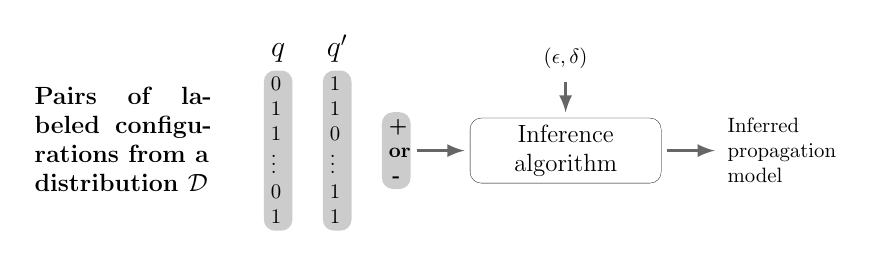
\begin{tikzpicture}
[scale=.75,auto,transform shape,
edge/.style={black!60,>=latex, shorten >=2pt, shorten <=2pt, line width=.4mm},
block/.style={draw=black,ultra thin,rounded corners},
conf/.style={fill=black!20,rounded corners}]
%%
\node[conf] (q) {\parbox{.25cm}{0\\1\\1\\$\vdots$\\0\\1}};
\node[anchor=south] at (q.north) {\Large $q$};
\node[right of=q,conf] (qp) {\parbox{.25cm}{1\\1\\0\\$\vdots$\\1\\1}};
\node[anchor=south] at (qp.north) {\Large $q'$};
\node[right of=qp,conf] (lab) {\parbox{.25cm}{\centering \bf +\\or\\-}};
%%
\node [left of=q,shift={(0,1.2)},font=\large,anchor=north east] {\parbox{3cm}{\bf
Pairs of labeled configurations from a\\ distribution $\mathcal{D}$}};
\node (inf) [block,right=of lab,font=\large] {\parnode{Inference algorithm}};
\node (result) [right=of inf] {\parbox{2cm}{Inferred propagation model}};
%%
\draw[edge,->] (lab) -- (inf);
\draw[edge,->] (inf) -- (result);
\draw[edge,<-] (inf.north) -- +(0,.7) node [anchor=south,black]
{$(\epsilon,\delta)$};
\end{tikzpicture}
\end{document}
